\section{Backend}
\subsection{Technologies and libraries}
\subsubsection{NodeJs}
Node.js is an open-source, cross-platform, back-end JavaScript runtime environment that runs on the
V8 engine and executes JavaScript code outside a web browser. Node.js lets developers use JavaScript
to write command line tools and for server-side scripting—running scripts server-side to produce
dynamic web page content before the page is sent to the user’s web browser. Consequently, Node.js
represents a "JavaScript everywhere" paradigm, unifying web-application development around a single
programming language, rather than different languages for server-side and client-side scripts.
\begin{itemize}
    \item \textbf{Used Version:}
\end{itemize}
\subsubsection{Serverless Framework}
The Serverless Framework is a free and open-source web framework written using Node.js. Serverless is the first
framework developed for building applications on AWS Lambda, a serverless computing platform provided
by Amazon as a part of Amazon Web Services.
\begin{itemize}
    \item \textbf{Used Version:}
\end{itemize}
\subsubsection{Amazon DynamoDB}
Amazon DynamoDB is a fully managed, multi-region, multi-active, durable, proprietary NoSQL database service that supports key-value
and document data structures and is offered by Amazon.com as part of the Amazon Web Services
portfolio.
\subsection{Architecture}
\subsubsection{Main components}
\subsubsection{External services}
\subsubsubsection{Amazon API Gateway}
Amazon API Gateway is a fully managed service that makes it easy for developers to create, publish, maintain, monitor,
and secure APIs at any scale. APIs act as the "front door" for applications to access data, business logic,
or functionality from your backend services. Using API Gateway, you can create RESTful APIs and WebSocket APIs that
enable real-time two-way communication applications. API Gateway supports containerized and serverless workloads,
as well as web applications.
\subsubsubsection{Amazon Cognito}
Amazon Cognito lets you add user sign-up, sign-in, and access control to your web and mobile apps quickly and easily.
Amazon Cognito scales to millions of users and supports sign-in with social identity providers, such as Apple,
Facebook, Google, and Amazon, and enterprise identity providers via SAML 2.0 and OpenID Connect.
\subsubsubsection{AWS Lambda}
AWS Lambda is an event-driven, serverless computing platform provided by Amazon as a part of Amazon Web Services.
It is a computing service that runs code in response to events and automatically manages the computing resources required by that code.
\subsubsubsection{Amazon S3}
Amazon Simple Storage Service (Amazon S3) is an object storage service that offers industry-leading scalability,
data availability, security, and performance.
\subsubsubsection{Stripe}
Stripe is a service that allows developers to integrate secure payment processing into their websites and applications.
\subsection{General description}
The functionalities provided by the platform permitted to identify the following domains:
\begin{itemize}
    \item \textbf{Carts};
    \item \textbf{Products};
    \item \textbf{Orders};
    \item \textbf{Tags};
    \item \textbf{Categories}.
\end{itemize}
The architecture is based on the following microservices:
\begin{itemize}
    \item \textbf{Carts service};
    \item \textbf{Products service};
    \item \textbf{Orders service};
    \item \textbf{Tags service};
    \item \textbf{Categories service}.
\end{itemize}
Microservices are independently deployable and allow for more team autonomy, CONTINUARE **********
\pagebreak
\subsection{Microservices structure}
Inserire testo se serve
\subsubsection{Carts service}
\begin{figure}[!h]
    \vspace{5px}
    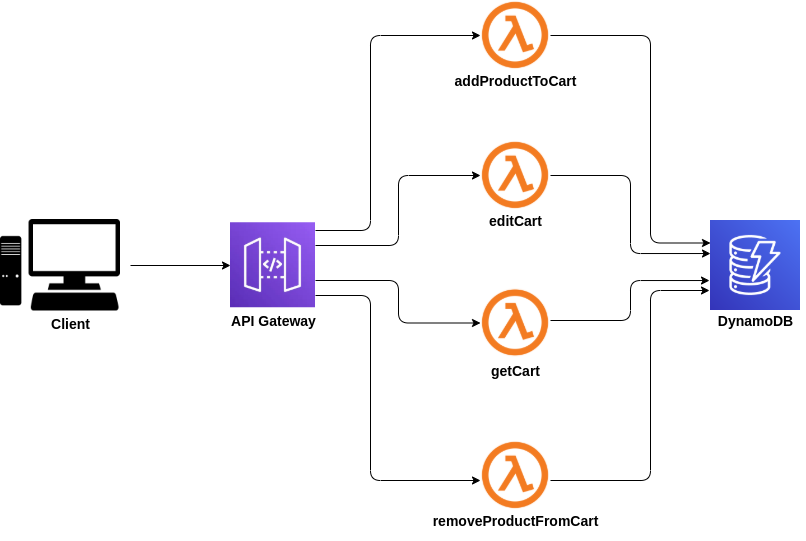
\includegraphics[scale=0.5]{../../../../Images/Diagrammi/maintainerManual/cartService.png}
    \centering
    \caption{Carts service}
\end{figure}
This microservice allows the user to:
\begin{itemize}
    \item Add a product to the cart;
    \item Remove a product from the cart;
    \item Modify the quantity of the items in the cart;
    \item View the items in the cart,
    \item Check out.
\end{itemize}
\pagebreak
\subsubsection{Products service}
\begin{figure}[!h]
    \vspace{5px}
    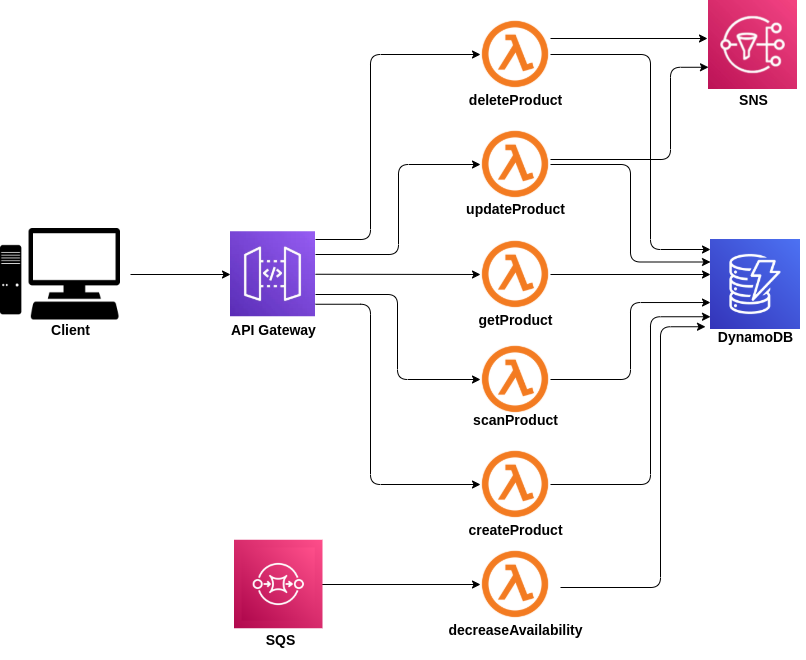
\includegraphics[scale=0.5]{../../../../Images/Diagrammi/maintainerManual/productService.png}
    \centering
    \caption{Products service}
\end{figure}
This microservice allows the user to:
\begin{itemize}
    \item Create a new product;
    \item Delete a product;
    \item View the product details;
    \item Find a specific product using filters;
    \item Modify informations about a product.
\end{itemize}
\pagebreak
\subsubsection{Orders service}
\begin{figure}[!h]
    \vspace{5px}
    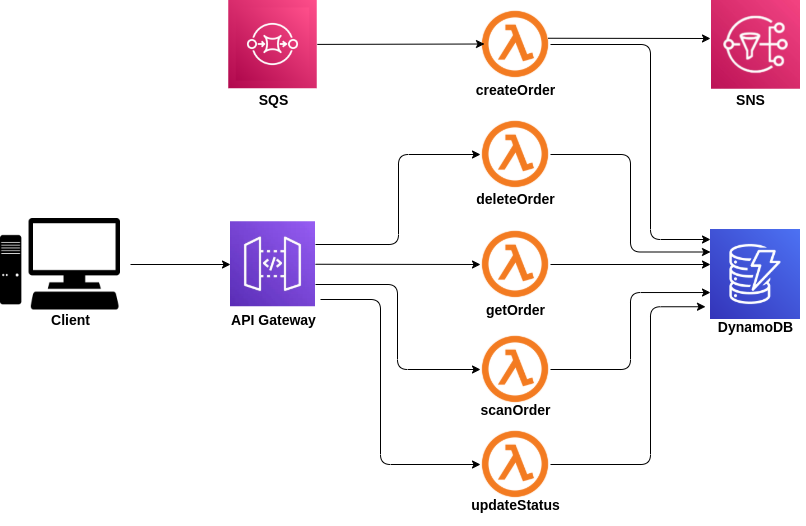
\includegraphics[scale=0.5]{../../../../Images/Diagrammi/maintainerManual/orderService.png}
    \centering
    \caption{Orders service}
\end{figure}
This microservice allows the user to:
\begin{itemize}
    \item Create a new order;
    \item Delete a order;
    \item View the order details;
    \item Find a specific order using filters.
\end{itemize}
\pagebreak
\subsubsection{Tags service}
\begin{figure}[!h]
    \vspace{5px}
    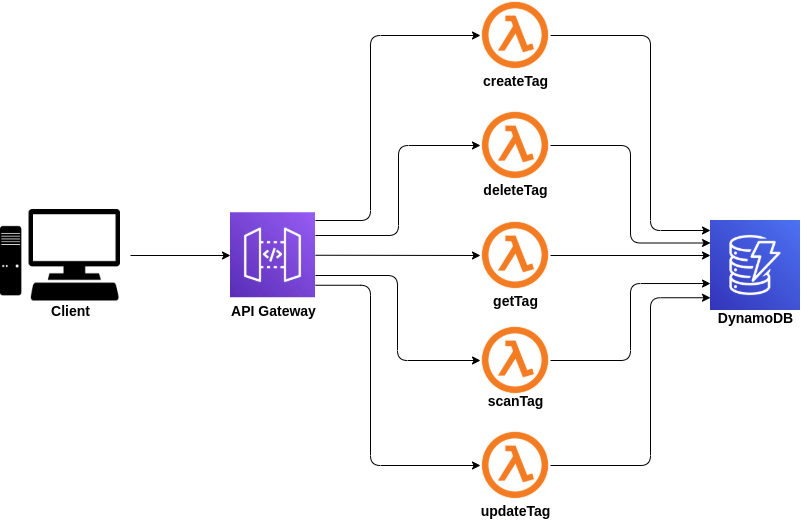
\includegraphics[scale=0.5]{../../../../Images/Diagrammi/maintainerManual/tagsService.png}
    \centering
    \caption{Tags service}
\end{figure}
This microservice allows the user to:
\begin{itemize}
    \item Create a new tag;
    \item Delete a tag;
    \item View the tag details;
    \item Find a specific tag using filters;
    \item Modify informations about a tag.
\end{itemize}
\pagebreak
\subsubsection{Categories service}
\begin{figure}[!h]
    \vspace{5px}
    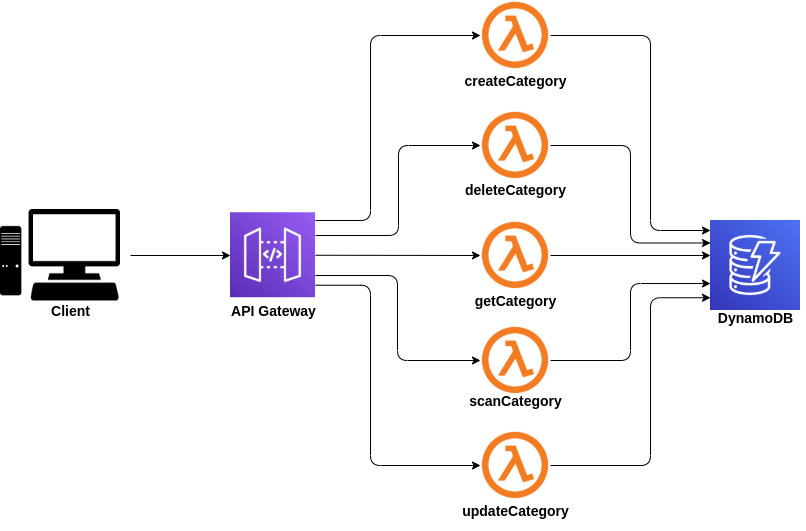
\includegraphics[scale=0.5]{../../../../Images/Diagrammi/maintainerManual/categoriesService.png}
    \centering
    \caption{Categories service}
\end{figure}
This microservice allows the user to:
\begin{itemize}
    \item Create a new category;
    \item Delete a category;
    \item View the category details;
    \item Find a specific category using filters;
    \item Modify informations about a category.
\end{itemize}
\pagebreak
\subsubsection{Images service}
\begin{figure}[!h]
    \vspace{5px}
    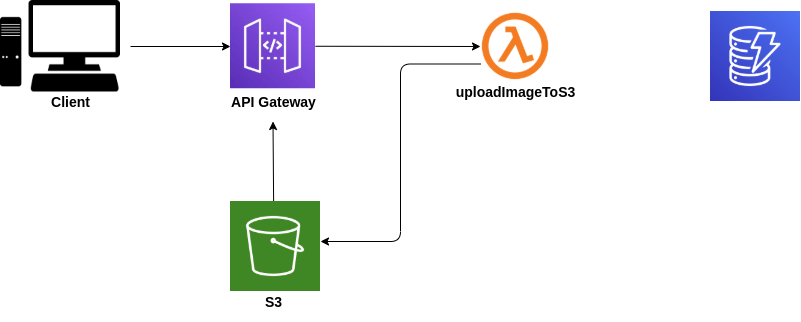
\includegraphics[scale=0.5]{../../../../Images/Diagrammi/maintainerManual/imageService.png}
    \centering
    \caption{Images service}
\end{figure}
This microservice allows the user to:
\begin{itemize}
    \item Update the image of a product.
\end{itemize}

\subsection{Class diagrams}
\subsection{Sequence diagrams}
The following sequence diagrams describe the main operations that can be carried out inside the platform:
\subsubsection{Create product}
\begin{figure}[!h]
    \vspace{5px}
    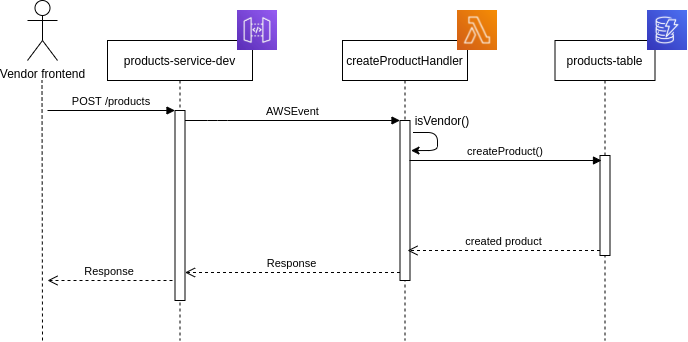
\includegraphics[scale=0.5]{../../../../Images/Diagrammi/maintainerManual/createProductSequence.png}
    \centering
    \caption{sequence diagram for creating a product} 
\end{figure}
\pagebreak
\subsubsection{Remove product from cart}
\begin{figure}[!h]
    \vspace{5px}
    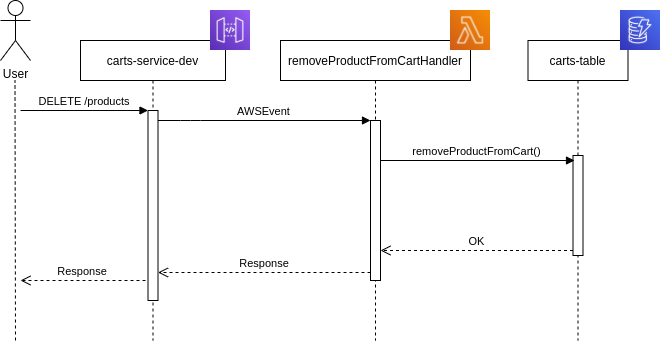
\includegraphics[scale=0.5]{../../../../Images/Diagrammi/maintainerManual/removeProductFromCart.png}
    \centering
    \caption{sequence diagram for removing a product from the cart} 
\end{figure}